\usetikzlibrary{arrows.meta, calc, fit, backgrounds, positioning}

\chapter[Implementación]{Implementación}
\label{ch:implementacion}

\insertminitoc
\parindent0pt

El presente capítulo describe el diseño y la implementación del sistema propuesto. Se
presenta en primer lugar la arquitectura general del sistema, que organiza sus
componentes en dos pipelines diferenciados según la dirección de comunicación. A
continuación se detallan los flujos de operación de cada pipeline mediante diagramas
de secuencia que muestran la interacción entre los módulos en tiempo de ejecución.
Finalmente se describe la integración de todos los componentes en la aplicación móvil
desarrollada con Flutter.

\section{Diseño de la Solución Tecnológica}

El sistema se estructura en dos pipelines complementarios que operan sobre el mismo
dispositivo físico y comparten una interfaz de usuario unificada. El primer pipeline
traduce las señas del \acrshort{lesho} ejecutadas por el niño sordo a texto en español,
permitiendo que la persona oyente lea en pantalla el mensaje comunicado. El segundo
pipeline convierte texto escrito en español en una representación visual de la seña
correspondiente, permitiendo que la persona oyente comunique mensajes al niño sordo
mediante el propio \acrshort{lesho}.

Ambos pipelines procesan la información íntegramente en el dispositivo, sin transmitir
datos a servidores externos. Esta decisión de diseño garantiza el funcionamiento sin
conexión a internet y protege la privacidad de los usuarios, dado que ninguna imagen
de cámara abandona el dispositivo en ningún momento.

\subsection{Arquitectura General del Sistema}

La arquitectura del sistema se organiza en cinco capas funcionales. La capa de captura
recibe la imagen de la cámara frontal del dispositivo a aproximadamente 30 fotogramas
por segundo. La capa de extracción de características aplica MediaPipe Hands sobre
cada fotograma para obtener las coordenadas tridimensionales de los 21 landmarks de
cada mano, que se normalizan respecto a la posición de la muñeca para producir un
vector de 126 valores correspondiente a las dos manos. En la ruta dinámica se ejecuta
además MediaPipe Pose para ubicar las manos respecto al cuerpo. La capa de inferencia
contiene los dos modelos de clasificación: el Modelo A, una red convolucional en una
dimensión (\acrshort{cnn} 1D) que clasifica una ventana de 20 fotogramas en 33 clases, y
el Modelo B, una red \acrshort{lstm} que clasifica secuencias en 50 señas dinámicas. La
capa de control implementa el filtro de persistencia temporal, la lógica de
activación del Modelo B mediante el control de grabación en pantalla, y el período de
enfriamiento tras cada detección. La capa de presentación es la interfaz de usuario construida en
Flutter, que muestra los resultados del reconocimiento y gestiona la animación del
muñeco que representa las señas en el pipeline de texto a seña.

La \autoref{fig:figure-arquitectura-lesho} muestra la organización de ambos pipelines
dentro del sistema, los componentes que los integran y las rutas de datos entre ellos.

\begin{figure}[H]
\centering
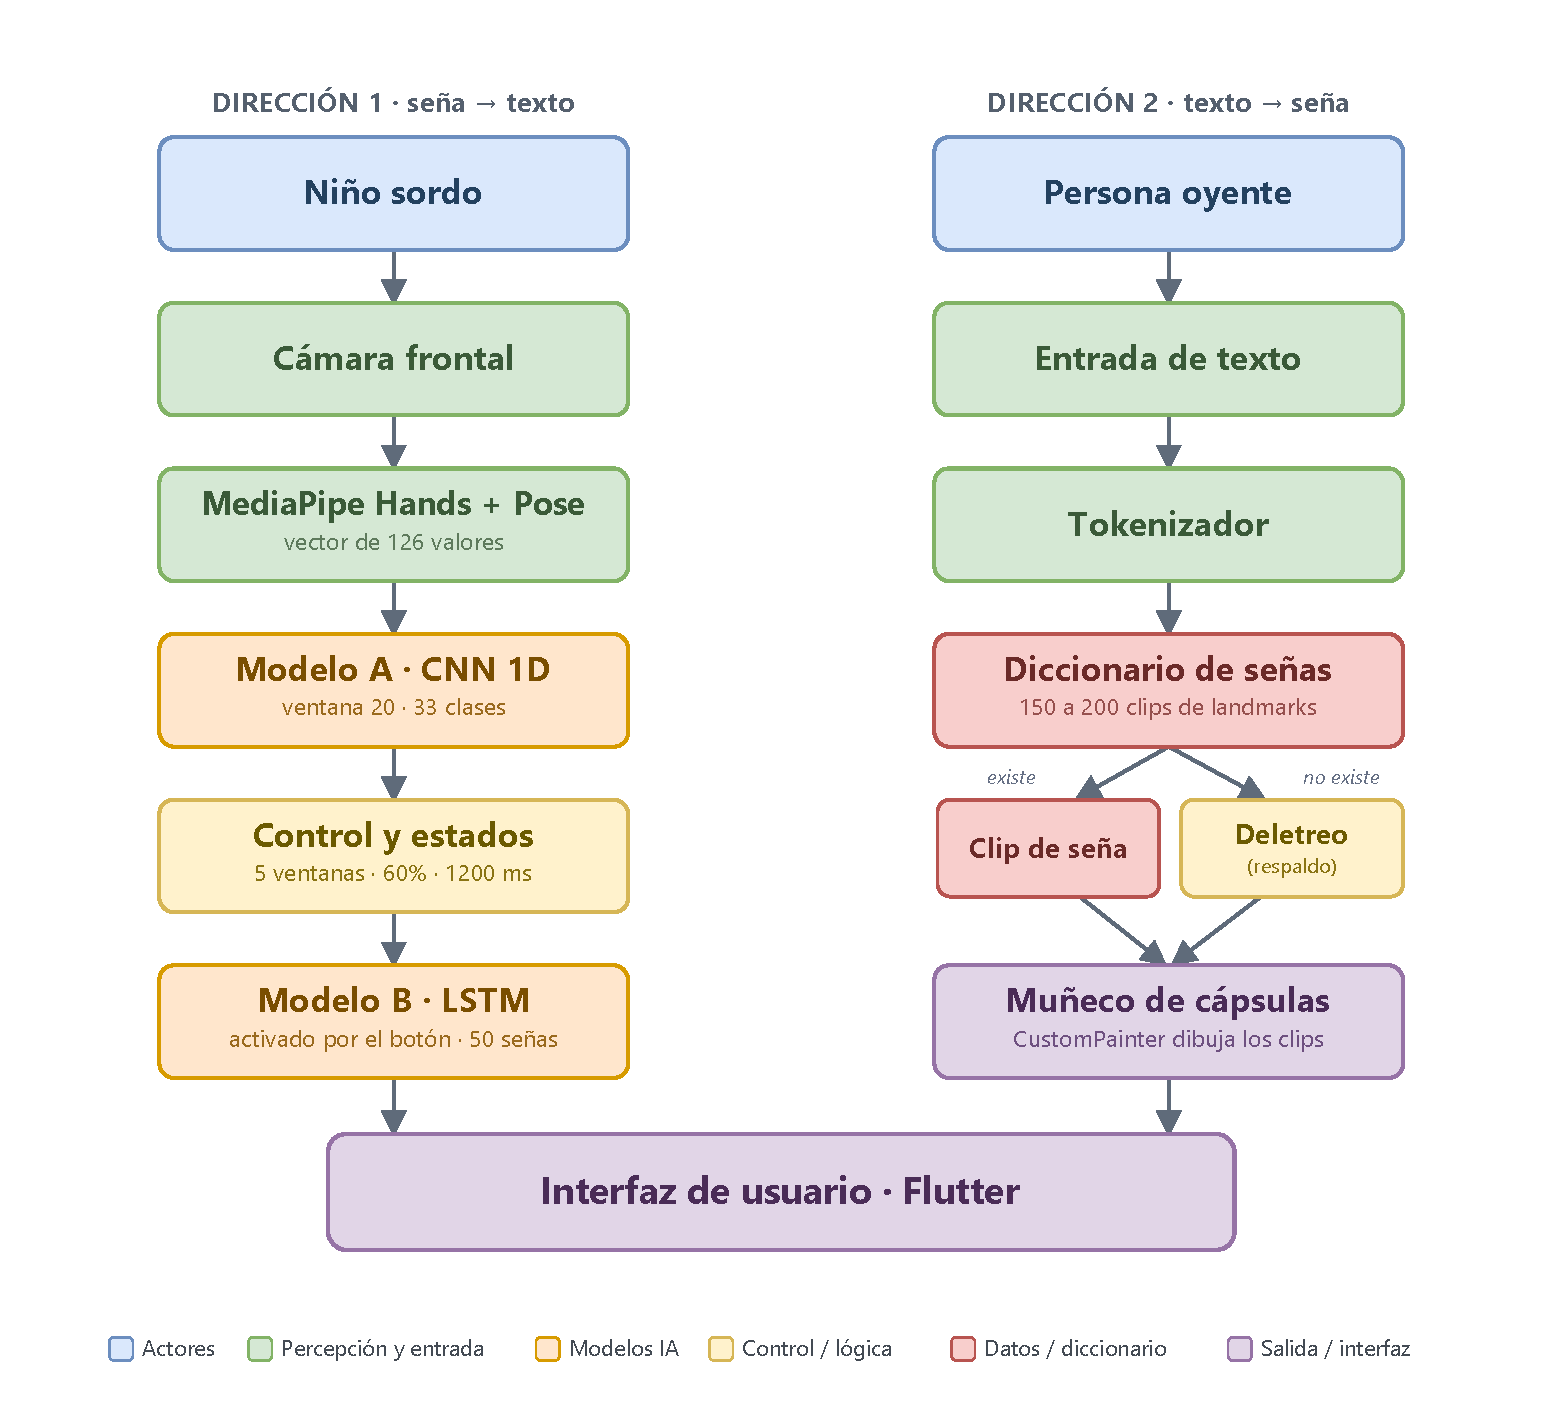
\includegraphics[width=\textwidth]{Figures/Implementacion/arquitectura.pdf}
\caption[Arquitectura general del sistema de comunicación LESHO]{Arquitectura general del sistema de comunicación \acrshort{lesho}. Se muestran los dos pipelines de comunicación y su convergencia en la interfaz de usuario compartida. Todo el procesamiento ocurre en el dispositivo, sin conexión a internet. Fuente: Elaboración propia.}
\label{fig:figure-arquitectura-lesho}
\end{figure}

La \autoref{fig:figure-arquitectura-lesho} deja ver que ambos pipelines comparten el
dispositivo y convergen en una interfaz común, pero recorren rutas independientes. En la
Dirección 1, el flujo desciende desde la cámara frontal hasta el Modelo B: cada capa entrega
su resultado a la siguiente, y el módulo de control acumula en el deletreo las letras que
el Modelo A confirma, o bien abre la ventana de grabación de una seña dinámica cuando la
persona usuaria acciona el control de grabación. En la Dirección 2, el texto escrito se descompone en la
secuencia de señas correspondiente y se entrega al muñeco de cápsulas, que la reproduce de
forma visual; cuando una palabra no existe en el diccionario, el sistema recurre al deletreo
letra por letra. Esta separación en dos rutas permite optimizar cada dirección por separado:
la primera prioriza la latencia del reconocimiento en tiempo real, mientras que la segunda
prioriza la claridad de la representación. El hecho de que ambas rutas se ejecuten por
completo en el dispositivo, sin depender de un servidor externo, es lo que garantiza el
funcionamiento sin conexión a internet y protege la privacidad de las imágenes capturadas por
la cámara, que nunca abandonan el teléfono.

\subsection{Vista Funcional del Sistema}

Más allá de su estructura interna, el sistema puede entenderse desde la experiencia de sus
dos usuarios. La \autoref{fig:figure-funcional} resume el recorrido funcional de cada
dirección de comunicación, con los pasos que percibe el usuario desde la acción inicial hasta
el resultado visible.

\begin{figure}[H]
\centering
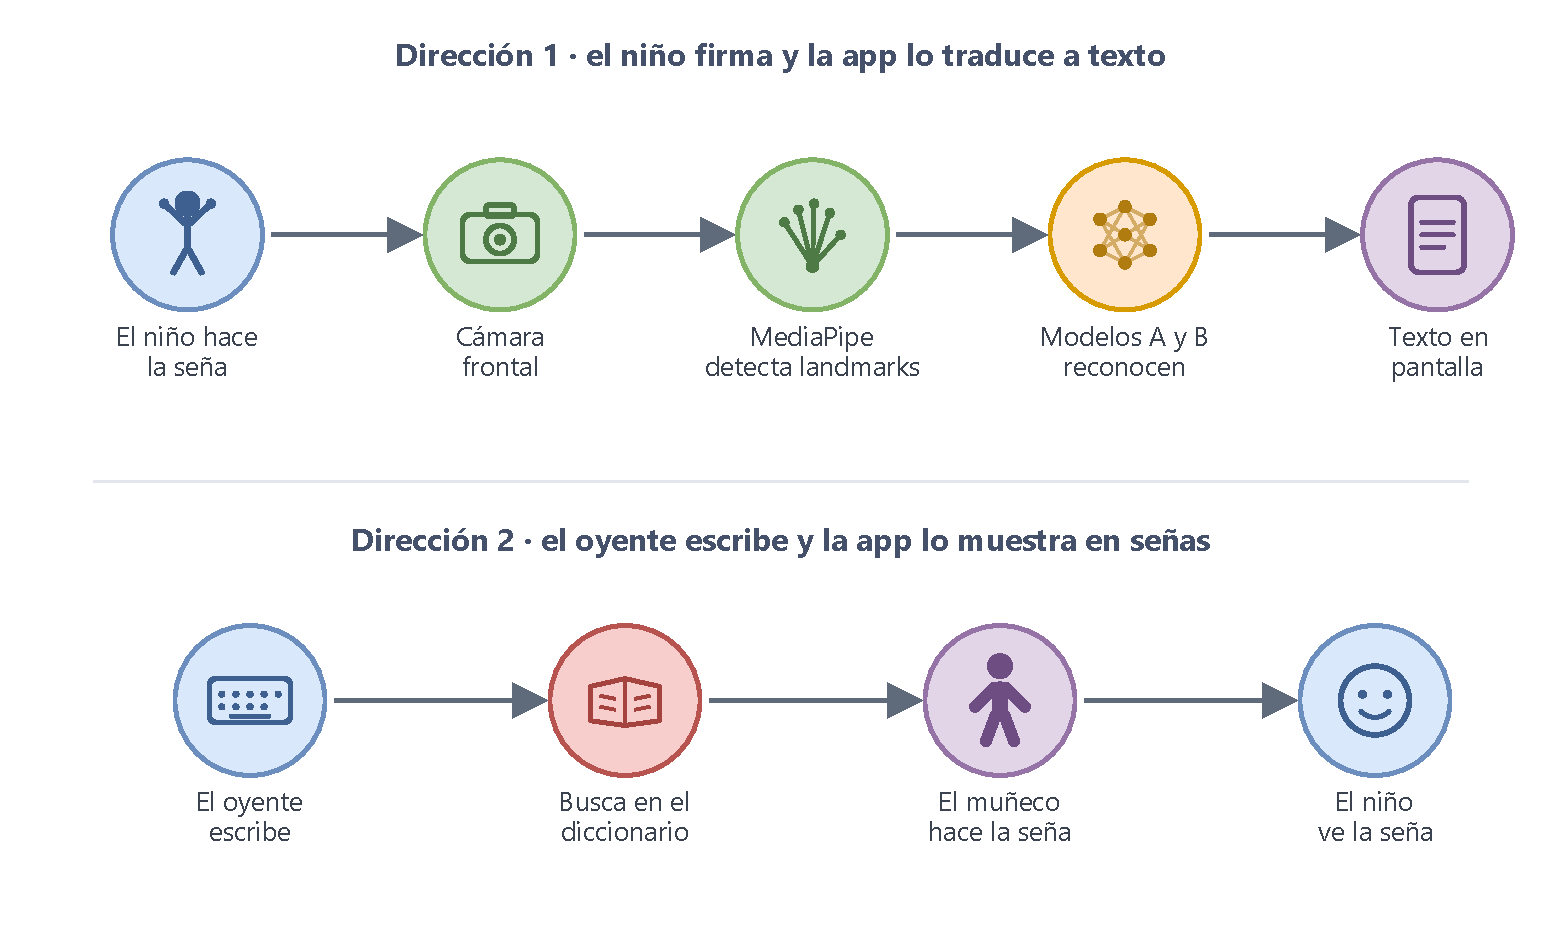
\includegraphics[width=\textwidth]{Figures/Implementacion/funcional.pdf}
\caption[Vista funcional del sistema LESHO]{Vista funcional del sistema. Se representan las dos direcciones de comunicación como flujos de operación: en la Dirección 1 el niño ejecuta la seña, la cámara la capta, MediaPipe extrae los landmarks, los modelos A y B la reconocen y el resultado aparece como texto; en la Dirección 2 la persona oyente escribe, la aplicación consulta el diccionario, el muñeco de cápsulas ejecuta la seña y el niño la observa. Fuente: Elaboración propia.}
\label{fig:figure-funcional}
\end{figure}

En la Dirección 1, el niño sordo inicia la comunicación: firma frente a la cámara y el sistema
traduce sus gestos a texto. El deletreo transcurre sin que deba tocar la pantalla, mientras
que para una seña completa delimita la grabación con el control correspondiente. En la Dirección 2, es la persona
oyente quien inicia el intercambio al escribir un mensaje que la aplicación convierte en señas
visibles para el niño. Ambos flujos comparten el mismo dispositivo y la misma interfaz, de modo
que la conversación puede alternar entre una dirección y la otra de forma natural. Esta lectura
funcional complementa la vista estructural de la arquitectura: mientras aquella muestra qué
componentes existen, esta muestra cómo se encadenan durante el uso real.

\subsection{Flujo de Reconocimiento de Señas}

El pipeline de reconocimiento de señas opera en tiempo real sobre el flujo continuo
de fotogramas capturados por la cámara frontal. Cada fotograma transita por un conjunto
de etapas que se ejecutan dentro del mismo ciclo de procesamiento antes de producir una
salida visible en pantalla.

En la primera etapa, MediaPipe Hands analiza el fotograma y extrae las coordenadas
tridimensionales de los 21 landmarks de cada mano detectada. Las coordenadas se
normalizan en dos pasos, restando la posición de la muñeca y dividiendo luego por el
tamaño de la mano, lo que produce un vector de 126 valores independiente de la posición
absoluta de las manos en la imagen y de su distancia a la cámara. Si no se detecta
ninguna mano con confianza suficiente, el fotograma se descarta.

Los vectores normalizados se acumulan en una ventana rodante de los últimos 20
fotogramas, que se entrega al Modelo A. El modelo devuelve una distribución de
probabilidad sobre las 33 clases. El módulo de control aplica entonces el
filtro de persistencia temporal: la misma clase debe aparecer como predicción
dominante durante al menos 5 ventanas consecutivas con una confianza igual o
superior al 60\,\% para que se confirme una detección. Una vez confirmada, se activa un
período de enfriamiento de 1200 milisegundos durante el cual no se aceptan nuevas
detecciones. El resultado de la detección determina el siguiente paso: si la clase
corresponde a una letra, se añade al buffer de texto visible en pantalla, y si es REPOSO
no se produce ninguna acción.

El reconocimiento de señas dinámicas sigue una ruta distinta, que la persona usuaria
delimita de forma explícita. Al pulsar el botón de grabación, el módulo de control activa
el modo dinámico y comienza a acumular la secuencia de vectores de landmarks; al pulsarlo
de nuevo para detener, envía la secuencia acumulada al Modelo B, que devuelve la seña
reconocida entre las 50 clases de su vocabulario.

La \autoref{fig:figure-secuencia-senas} muestra la interacción entre los componentes
del sistema durante el reconocimiento, incluyendo la bifurcación de comportamiento
según la clase detectada por el Modelo A.

\begin{figure}[H]
\centering
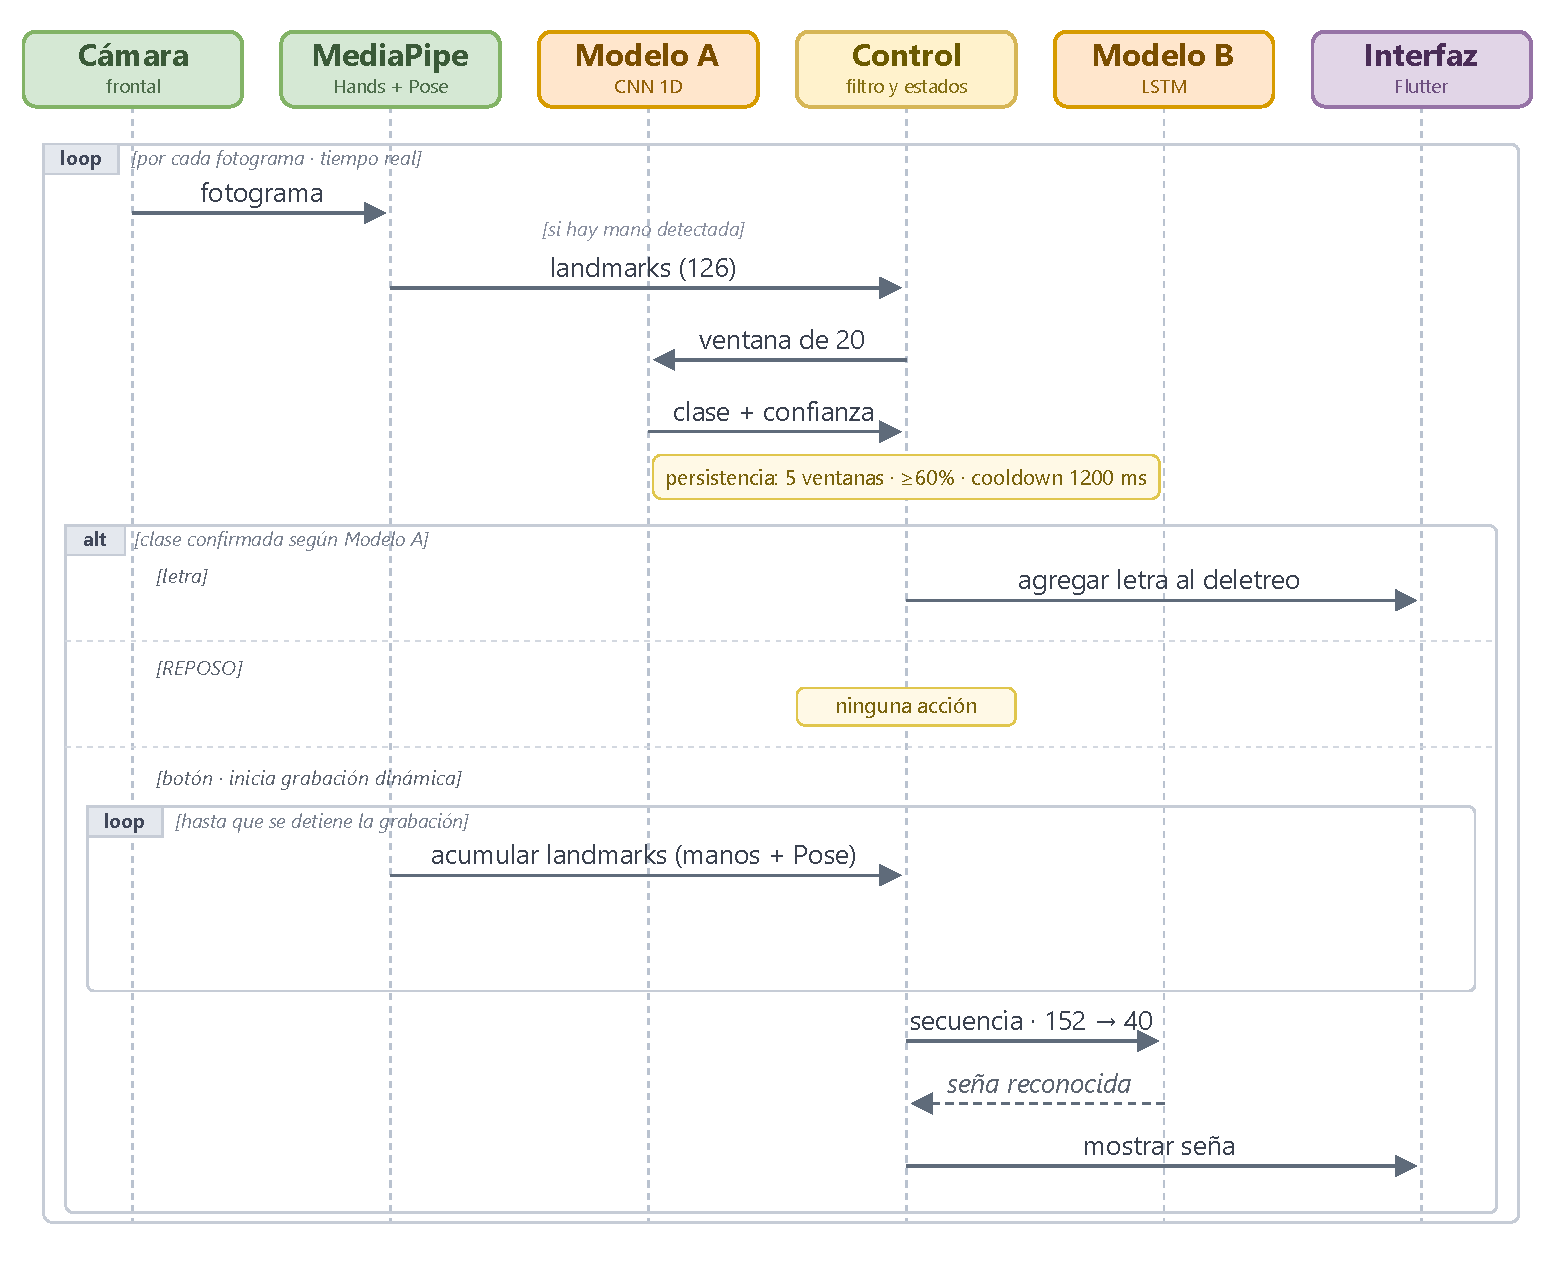
\includegraphics[width=\textwidth]{Figures/Implementacion/secuencia.pdf}
\caption[Flujo de reconocimiento de señas del sistema LESHO]{Flujo de reconocimiento de señas. El diagrama de secuencia muestra cómo el módulo de control orquesta el reconocimiento en tiempo real: recibe los landmarks de MediaPipe, arma la ventana que clasifica el Modelo A y, según la clase confirmada, agrega una letra al deletreo, no ejecuta ninguna acción ante un reposo, o abre el ciclo de grabación dinámica que acumula fotogramas hasta que la persona usuaria detiene la grabación, momento en el que el Modelo B produce la seña reconocida. Fuente: Elaboración propia.}
\label{fig:figure-secuencia-senas}
\end{figure}

En el diagrama se aprecia que el módulo de control es el eje del reconocimiento: recibe
los landmarks de MediaPipe, mantiene la ventana rodante que entrega al Modelo A y, con la
respuesta de este, aplica el filtro de persistencia antes de actuar. La rama de la
grabación dinámica es la más compleja, porque abre un ciclo en el que cada fotograma se
acumula para el Modelo B hasta que la persona usuaria cierra la grabación; solo entonces
se ejecuta la inferencia de la seña dinámica. Este diseño evita que el Modelo B, más
costoso, se ejecute de forma continua, y reserva su uso para el momento exacto en que hay
una seña completa que interpretar.

\subsection{Flujo de Texto a Seña}

El pipeline de texto a seña permite que la persona oyente comunique mensajes en
español al niño sordo utilizando el propio \acrshort{lesho}. El proceso se inicia cuando el
oyente escribe texto en el campo de entrada de la aplicación y confirma el envío.

La aplicación tokeniza el texto en palabras individuales y procesa cada una de forma
secuencial. Para cada palabra, consulta el diccionario de señas. Si existe un clip
correspondiente a esa palabra, se encola para reproducción. Si la palabra no está
registrada en el diccionario, el sistema activa el mecanismo de respaldo: la palabra se
descompone en letras y cada letra se busca individualmente en el diccionario, que
siempre contiene las 30 letras del alfabeto dactilológico del \acrshort{lesho}. Los clips
resultantes se reproducen en secuencia sobre el muñeco en la pantalla del dispositivo,
orientada hacia el niño sordo.

La \autoref{fig:figure-secuencia-texto} muestra el flujo completo del pipeline de
texto a seña, incluyendo la bifurcación entre el camino principal y el mecanismo de
respaldo por deletreo.

\begin{figure}[H]
\centering
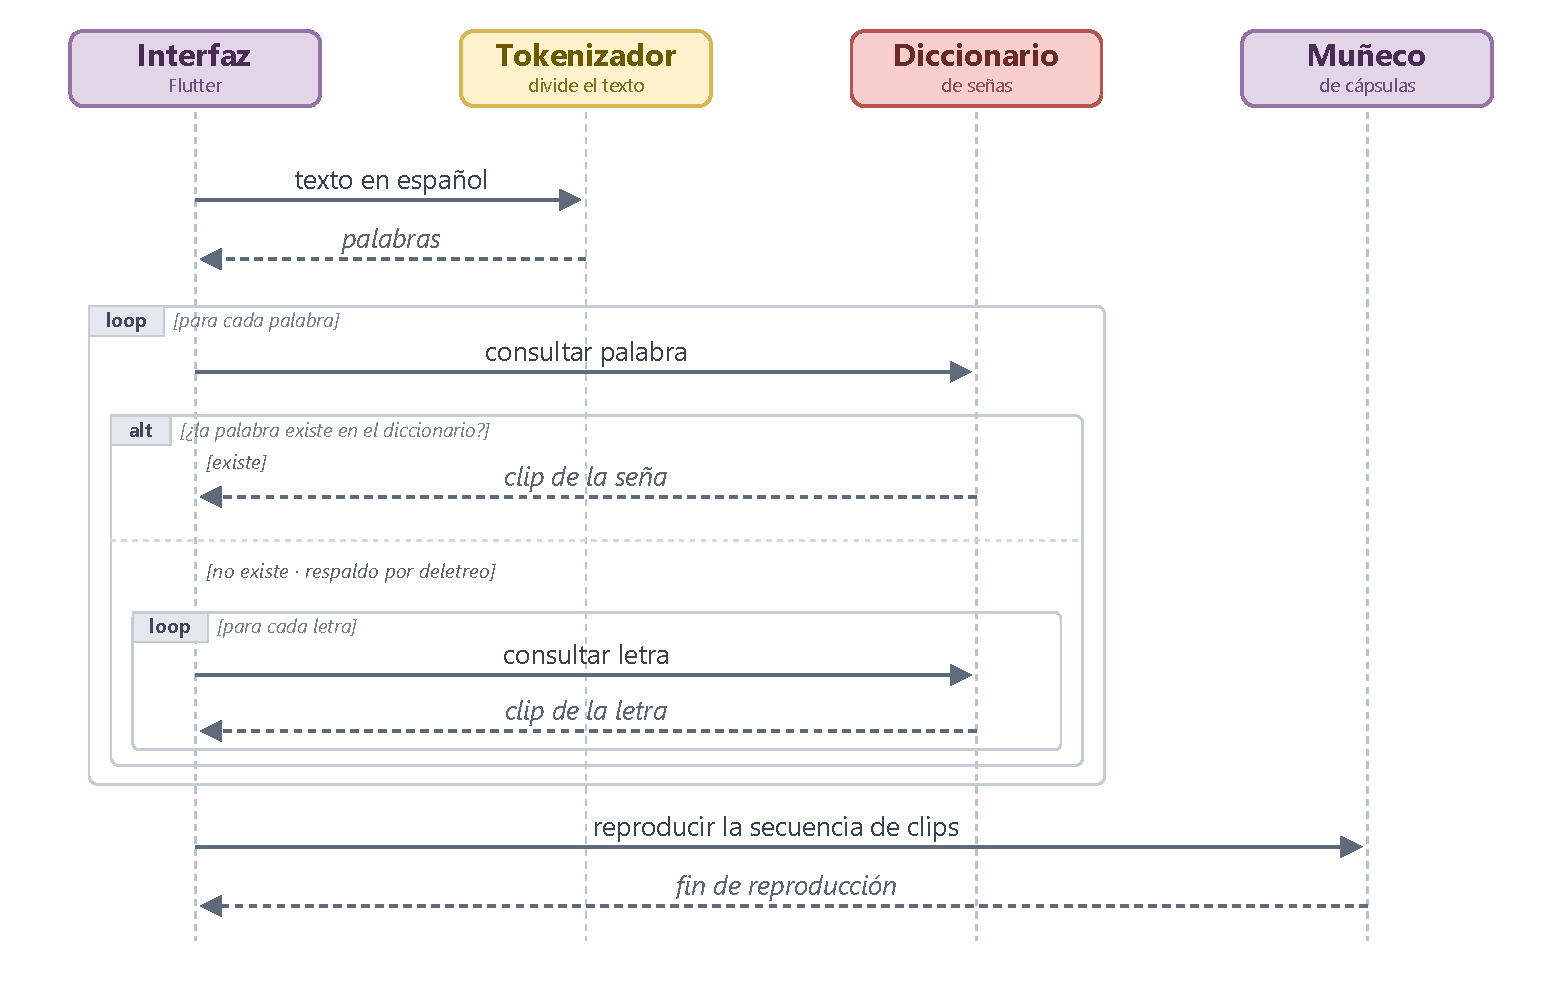
\includegraphics[width=\textwidth]{Figures/Implementacion/texto_sena.pdf}
\caption[Flujo del pipeline de texto a seña del sistema LESHO]{Flujo de texto a seña. El diagrama de secuencia muestra cómo la interfaz tokeniza el texto que escribe la persona oyente y, por cada palabra, consulta el diccionario de señas: si la palabra existe recupera el clip de su seña, y si no existe recurre al respaldo de deletreo, recuperando el clip de cada letra. Una vez reunida la secuencia, el muñeco de cápsulas la reproduce en pantalla. Fuente: Elaboración propia.}
\label{fig:figure-secuencia-texto}
\end{figure}

% ===========================================================================
\section{Implementación de la Aplicación Móvil}
\label{sec:implementacion-app}
% ===========================================================================

La aplicación se desarrolla con \textit{Flutter} como \textit{framework} multiplataforma,
utilizando \textit{Dart} como lenguaje de programación. Esta elección permite compilar
una única base de código para \textit{Android}, iOS y la web desde el mismo repositorio.
El objetivo principal de la implementación es \textit{Android}, dado que es la
plataforma predominante en el contexto hondureño. La distribución no requiere publicación
en tiendas de aplicaciones oficiales: la aplicación se empaqueta como un archivo
\acrfull{apk} instalable directamente en el dispositivo.

% ---------------------------------------------------------------------------
\subsection{Estructura del Proyecto}
\label{sec:estructura-proyecto}
% ---------------------------------------------------------------------------

El repositorio se organiza en dos partes diferenciadas. La parte de la aplicación
móvil contiene el código \textit{Flutter}, los modelos exportados a formato
\acrshort{tflite} empaquetados como \textit{assets}, los archivos de etiquetas y los
clips de landmarks del diccionario de señas. La parte del \textit{pipeline} de
entrenamiento contiene los \textit{scripts} de captura, preprocesamiento y entrenamiento
en \textit{Python}, junto con el conjunto de datos en formato \textit{CSV}.

Los paquetes principales de los que depende la aplicación son: el paquete
\texttt{camera}, para la captura del flujo de video en tiempo real desde la cámara
frontal; y el paquete \texttt{tflite\_flutter}, para la ejecución de inferencia con los
modelos clasificadores dentro del proceso de \textit{Dart}. La representación visual de
las señas en el módulo de texto a seña no utiliza un reproductor de video externo, sino
un muñeco animado que se dibuja directamente con el \textit{CustomPainter} de
\textit{Flutter} a partir de los clips de landmarks. Todos los \textit{assets} críticos
(modelos y clips) se incluyen dentro del paquete de la aplicación, lo que garantiza el
funcionamiento sin conexión a internet.

% ---------------------------------------------------------------------------
\subsection{Captura y Extracción de Características}
\label{sec:captura-landmarks}
% ---------------------------------------------------------------------------

La aplicación activa la cámara frontal del dispositivo mediante el paquete
\texttt{camera} y procesa el flujo de video a aproximadamente 30 fotogramas por
segundo. Cada fotograma se entrega a \textit{MediaPipe Hands}, que devuelve las
coordenadas tridimensionales de los 21 \textit{landmarks} de la mano detectada.
La integración de \textit{MediaPipe} con \textit{Flutter} se realiza mediante un
canal de plataforma (\textit{platform channel}) que ejecuta \textit{MediaPipe} en un
hilo nativo en segundo plano, de modo que el hilo de la interfaz permanece libre y la
captura no se bloquea.

Cada mano detectada aporta 21 \textit{landmarks} con 3 coordenadas ($x$, $y$, $z$), de
modo que las dos manos conforman un vector de 126 valores. Antes de entregarlos a los
modelos, los valores se normalizan en dos pasos. Primero se restan las coordenadas del
\textit{landmark} 0, correspondiente a la muñeca, de cada mano, con lo que el vector
resultante deja de depender de la posición absoluta de las manos dentro del cuadro de la
cámara. Después se divide por el tamaño de la mano, con lo que tampoco depende de la
distancia a la que se encuentre el usuario. Ambas operaciones incrementan la robustez del
clasificador ante distintas posiciones del dispositivo y del usuario. En la ruta de señas dinámicas se ejecuta además
\textit{MediaPipe Pose}, que aporta la ubicación de las manos respecto al cuerpo. Si
\textit{MediaPipe Hands} no detecta ninguna mano con confianza suficiente en un
fotograma dado, ese fotograma se descarta y no se entrega a ninguno de los modelos.

% ---------------------------------------------------------------------------
\subsection{Módulo de Reconocimiento de Señas}
\label{sec:modulo-reconocimiento}
% ---------------------------------------------------------------------------

El módulo de reconocimiento de señas implementa el \textit{pipeline} de la
Dirección 1 del sistema y opera de forma continua sobre el flujo de fotogramas
procesados por \textit{MediaPipe}.

\subsubsection{Inferencia con el Modelo A}

Los vectores normalizados de 126 valores se acumulan en una ventana rodante de 20
fotogramas que se entrega al Modelo A, implementado como una red convolucional 1D
(\acrshort{cnn} 1D) y ejecutado mediante \acrshort{tflite}. El modelo devuelve una
distribución de probabilidad sobre las 33 clases con que fue entrenado: las 30 letras del
alfabeto dactilológico del \acrshort{lesho}, la clase de reposo y las dos señas de control
que se evaluaron durante el desarrollo y que la versión final no utiliza. La clase
con mayor probabilidad constituye la predicción de la ventana actual. Clasificar una
ventana y no un fotograma aislado es lo que permite reconocer las cinco letras que se
ejecutan con movimiento: la J, la Ñ, la Z, la LL y la RR.

\subsubsection{Filtro de Persistencia Temporal y Período de Enfriamiento}

El módulo de control no actúa sobre ninguna predicción individual. Mantiene un
contador de ventanas consecutivas en las que la misma clase aparece como predicción
dominante. Solo cuando esa clase acumula cinco ventanas consecutivas con una confianza
igual o superior al 60\,\% se confirma la detección. Tras la confirmación, se activa
un período de enfriamiento de 1200 milisegundos durante el cual el módulo ignora nuevas
predicciones. Este mecanismo evita detecciones repetidas causadas por la transición
lenta de la mano entre una seña y la siguiente.

\subsubsection{Máquina de Estados del Reconocimiento}

El módulo de control opera con dos estados diferenciados. En el estado de deletreo, el
sistema clasifica de forma continua la ventana rodante de fotogramas y actúa según la
clase confirmada: si es una letra, la añade al \textit{buffer} de texto visible en
pantalla, y si es REPOSO no produce ninguna acción. El módulo transita al estado de
grabación dinámica cuando la persona usuaria pulsa el control de grabación. En ese estado
el sistema acumula los vectores de \textit{landmarks} de fotogramas sucesivos en lugar de
clasificarlos por ventana. Al detener la grabación, el módulo entrega la secuencia
acumulada al Modelo B y regresa al estado de deletreo.

\subsubsection{Inferencia con el Modelo B}

El Modelo B, implementado como una red \acrshort{lstm} y ejecutado mediante
\acrshort{tflite}, recibe la secuencia acumulada durante la grabación. Cada
fotograma de la secuencia combina la configuración de las manos con la ubicación de
estas respecto al cuerpo, obtenida con \textit{MediaPipe Pose}, para conformar una
entrada de 152 valores; la secuencia se remuestrea a una longitud fija de 40 fotogramas
antes de la inferencia. El modelo devuelve una distribución de probabilidad sobre las
50 clases dinámicas del vocabulario reconocido. La seña con mayor probabilidad se
muestra en la interfaz como resultado del reconocimiento, y el sistema regresa al
estado de deletreo para continuar el ciclo.

% ---------------------------------------------------------------------------
\subsection{Módulo de Texto a Seña}
\label{sec:modulo-texto-sena}
% ---------------------------------------------------------------------------

El módulo de texto a seña implementa el \textit{pipeline} de la Dirección 2 del
sistema. La persona oyente ingresa un mensaje en español mediante un campo de texto
de la interfaz. El módulo divide el texto en palabras individuales mediante un
tokenizador que separa por espacios y descarta puntuación.

Para cada palabra resultante, el módulo consulta el diccionario de señas. Si la palabra
tiene un clip correspondiente en el diccionario, ese clip se añade a la cola de
reproducción. Si la palabra no se encuentra en el diccionario, el módulo la descompone
letra por letra y añade a la cola el clip de cada letra del alfabeto dactilológico,
aplicando así el mecanismo de respaldo por deletreo descrito en el diseño del sistema.
Una vez procesadas todas las palabras, el muñeco reproduce la cola de clips de forma
secuencial, mostrando cada seña de forma ordenada en pantalla.

El diccionario de señas tiene como objetivo entre 150 y 200 entradas, que incluyen
las 30 letras del alfabeto dactilológico, las 50 señas dinámicas del vocabulario del
Modelo B, y señas adicionales de vocabulario común agrupadas por categorías: números,
colores, vínculos familiares, emociones, entorno escolar y necesidades básicas.

% ---------------------------------------------------------------------------
\subsection{Interfaz de Usuario}
\label{sec:interfaz-usuario}
% ---------------------------------------------------------------------------

La interfaz de usuario se diseña considerando que el usuario principal es un niño
sordo. Los elementos interactivos tienen un tamaño generoso para facilitar la
interacción táctil, y la retroalimentación visual de cada acción es clara e
inmediata. La aplicación presenta dos pantallas principales: la pantalla de
reconocimiento, que muestra la vista de la cámara frontal y el texto acumulado del
deletreo o la seña dinámica reconocida, y la pantalla de texto a seña, donde la
persona oyente escribe el mensaje y la aplicación reproduce la secuencia de señas
correspondiente.

La transición entre pantallas es explícita y controlada por el usuario, de modo que
en cada momento solo uno de los dos \textit{pipelines} permanece activo. La
aplicación no requiere conexión a internet en ninguna de sus funciones, dado que los
modelos de clasificación y el diccionario de señas están empaquetados dentro del
\acrshort{apk}.

% ===========================================================================
\section{Pruebas y Resultados Preliminares}
% ===========================================================================

A lo largo de las semanas de desarrollo, el sistema no se armó de una sola vez, sino que se
fue construyendo y probando por partes. Esta sección recoge esas pruebas y los resultados
preliminares que arrojaron. Conviene aclararlo desde el inicio: son resultados obtenidos con
pocos datos, cuyo propósito fue orientar las decisiones de diseño y confirmar que cada pieza
funcionaba antes de invertir en la grabación del conjunto de datos definitivo. La evaluación
formal, con los cuatro participantes, se desarrolla en el capítulo de resultados.

El enfoque fue iterativo: cada componente se probó apenas estuvo integrado, con un conjunto
reducido de muestras y directamente sobre un teléfono real de gama baja, un Samsung Galaxy
A13. Así se pudo confirmar de forma temprana que la tubería completa funcionaba en el
dispositivo y detectar los problemas propios de la ejecución \textit{on-device} desde el
inicio, antes de escalar el conjunto de datos.

Durante estas semanas se llevaron al dispositivo los tres bloques del sistema. El deletreo del
alfabeto (Modelo A) se probó primero, pues utiliza una sola mano y no requiere MediaPipe Pose,
y funcionó de forma fluida en el teléfono. Enseguida se integró la tubería completa del Modelo
B, con MediaPipe Pose, el marco de referencia del cuerpo y el preprocesamiento de la secuencia;
esta tubería se validó comparando su salida en el teléfono contra la implementación de
referencia en \textit{Python}, para asegurar que ambas produjeran los mismos vectores. Para
probar el reconocimiento de señas dinámicas se entrenó un modelo reducido con diez palabras y
una sola persona, concebido como prueba de concepto de la tubería y no como un modelo
generalizable. Por último, la Dirección 2 se probó reproduciendo señas en el muñeco de cápsulas
sobre el mismo dispositivo.

Las pruebas con este conjunto reducido de datos evidenciaron lo siguiente:

\begin{itemize}
    \item El deletreo del alfabeto funciona de forma estable en el teléfono, con una respuesta
    suficientemente ágil para escribir letra por letra.
    \item El Modelo B aprende la tarea con los datos de una sola persona, alcanzando una
    exactitud de validación cercana al 99\,\%. Este valor confirma que la arquitectura y el
    preprocesamiento son correctos, pero es optimista: al provenir de una única persona, no
    anticipa el desempeño con personas nuevas.
    \item Las señas que se distinguen por el lugar de articulación se reconocen con solidez.
    Por ejemplo, HOSPITAL, que se ejecuta en una zona bien diferenciada, se identifica sin
    problema. En cambio, las señas que comparten lugar y difieren solo en la forma o el
    movimiento de la mano, como HOLA y AGUA, se confunden con facilidad y son las que más se
    benefician de contar con más datos y más personas.
\end{itemize}

Más allá de las cifras, estas pruebas dejaron aprendizajes que moldearon el diseño final. El
primero fue la importancia de incorporar la punta del índice a la ubicación de la mano en el
cuerpo: muchas señas se hacen apuntando con los dedos a una zona, como HOLA hacia la frente o
AGUA hacia la boca, mientras la muñeca permanece a un costado; sin la punta del índice, ambas
señas colapsaban en una sola. El segundo fue la corrección del factor de aspecto: el conjunto
de datos se grabó en formato 16:9 y el teléfono entrega 3:4, de modo que las coordenadas debían
corregirse en vivo según el aspecto real de la cámara, pues de lo contrario el modelo confundía
casi todas las señas. El tercero fue una limitación del hardware: el Samsung Galaxy A13 entrega
alrededor de cinco fotogramas por segundo cuando procesa dos manos junto con MediaPipe Pose, una
tasa baja que obliga a capturar la seña con cuidado y a sostener la posición inicial. El
deletreo, al usar una sola mano y no ejecutar Pose, no se ve afectado por esta limitación.

En conjunto, estos resultados preliminares validan la viabilidad técnica del sistema: la
tubería completa, desde la cámara hasta la clasificación y la representación en el muñeco,
funciona por entero en el dispositivo y sin conexión a internet. También delimitan con claridad
el trabajo que resta, que es ampliar el conjunto de datos a varias personas para que el
reconocimiento de señas dinámicas generalice más allá de las condiciones de grabación. Ese
conjunto de datos completo y su evaluación formal se presentan en el capítulo siguiente.
